\documentclass{beamer}

% Beamer style
%\usetheme[secheader]{Madrid}
\usetheme{CambridgeUS}
\usecolortheme[rgb={0.65,0.15,0.25}]{structure}
%\usefonttheme[onlymath]{serif}
\beamertemplatenavigationsymbolsempty
%\AtBeginSubsection

% Packages
%\usepackage[french]{babel}
\usepackage[latin1]{inputenc}
\usepackage{color}
\usepackage{dsfont, stmaryrd}
\usepackage{amsmath, amsfonts, amssymb}
\usepackage{stmaryrd}
\usepackage{epsfig}
\usepackage{url}
\usepackage{/Latex/astats}
%\usepackage[all]{xy}
\usepackage{graphicx}

% Commands
\definecolor{darkred}{rgb}{0.65,0.15,0.25}
\newcommand{\emphase}[1]{\textcolor{darkred}{#1}}
\newcommand{\paragraph}[1]{\emphase{#1}}
\newcommand{\refer}[1]{\textcolor{blue}{\sl \cite{#1}}}
\newcommand{\Refer}[1]{\textcolor{blue}{\sl #1}}
\newcommand{\newblock}{}

% Symbols
\newcommand{\Abf}{{\bf A}}
\newcommand{\Beta}{\text{B}}
\newcommand{\Bcal}{\mathcal{B}}
\newcommand{\BIC}{\text{BIC}}
\newcommand{\dd}{\text{d}}
\newcommand{\dbf}{{\bf d}}
\newcommand{\Dcal}{\mathcal{D}}
\newcommand{\Esp}{\mathbb{E}}
\newcommand{\Ecal}{\mathcal{E}}
\newcommand{\Gcal}{\mathcal{G}}
\newcommand{\Gam}{\mathcal{G}\mbox{am}}
\newcommand{\Ibb}{\mathbb{I}}
\newcommand{\Ibf}{{\bf I}}
\newcommand{\ICL}{\text{ICL}}
\newcommand{\Cov}{\mathbb{C}\text{ov}}
\newcommand{\Corr}{\mathbb{C}\text{orr}}
\newcommand{\Var}{\mathbb{V}}
\newcommand{\Vsf}{\mathsf{V}}
\newcommand{\pen}{\text{pen}}
\newcommand{\Fcal}{\mathcal{F}}
\newcommand{\Hbf}{{\bf H}}
\newcommand{\Hcal}{\mathcal{H}}
\newcommand{\Jcal}{\mathcal{J}}
\newcommand{\Kbf}{{\bf K}}
\newcommand{\Lcal}{\mathcal{L}}
\newcommand{\Mcal}{\mathcal{M}}
\newcommand{\mbf}{{\bf m}}
\newcommand{\mum}{\mu(\mbf)}
\newcommand{\Ncal}{\mathcal{N}}
\newcommand{\Nbf}{{\bf N}}
\newcommand{\Nm}{N(\mbf)}
\newcommand{\Ocal}{\mathcal{O}}
\newcommand{\Obf}{{\bf 0}}
\newcommand{\Omegas}{\underset{s}{\Omega}}
\newcommand{\Pbf}{{\bf P}}
\newcommand{\Pcal}{\mathcal{P}}
\newcommand{\Qcal}{\mathcal{Q}}
\newcommand{\Rbb}{\mathbb{R}}
\newcommand{\Rcal}{\mathcal{R}}
\newcommand{\sbf}{{\bf s}}
\newcommand{\Sbf}{{\bf S}}
\newcommand{\Scal}{\mathcal{S}}
\newcommand{\Ucal}{\mathcal{U}}
\newcommand{\Vcal}{\mathcal{V}}
\newcommand{\Tbf}{{\bf T}}
\newcommand{\ubf}{{\bf u}}
\newcommand{\Ubf}{{\bf U}}
\newcommand{\Wbf}{{\bf W}}
\newcommand{\xbf}{{\bf x}}
\newcommand{\Xbf}{{\bf X}}
\newcommand{\ybf}{{\bf y}}
\newcommand{\Ybf}{{\bf Y}}
\newcommand{\zbf}{{\bf z}}
\newcommand{\Zbf}{{\bf Z}}
\newcommand{\betabf}{\mbox{\mathversion{bold}{$\beta$}}}
\newcommand{\pibf}{\mbox{\mathversion{bold}{$\pi$}}}
\newcommand{\Sigmabf}{\mbox{\mathversion{bold}{$\Sigma$}}}
\newcommand{\gammabf}{\mbox{\mathversion{bold}{$\gamma$}}}
\newcommand{\mubf}{\mbox{\mathversion{bold}{$\mu$}}}
\newcommand{\nubf}{\mbox{\mathversion{bold}{$\nu$}}}
\newcommand{\Thetabf}{\mbox{\mathversion{bold}{$\Theta$}}}
\newcommand{\thetabf}{\mbox{\mathversion{bold}{$\theta$}}}
\newcommand{\BP}{\text{BP}}
\newcommand{\EM}{\text{EM}}
\newcommand{\VEM}{\text{VEM}}
\newcommand{\VBEM}{\text{VB}}
\newcommand{\cst}{\text{cst}}
\newcommand{\obs}{\text{obs}}
\newcommand{\ra}{\emphase{ $\rightarrow$~}}
\newcommand{\QZ}{Q_{Z}}
\newcommand{\Qt}{Q_{\theta}}

% Directory
\newcommand{\fignet}{/RECHERCHE/RESEAUX/Exposes/Figures}
\newcommand{\figmotif}{/RECHERCHE/RESEAUX/Motifs/FIGURES}


%====================================================================
\title{Estimating species abundance}

\author[S. Robin]{S. Li-Thiao-T�, J.-J. Daudin, \underline{S. Robin}}

\institute[AgroParisTech / INRA]{AgroParisTech / INRA \\
  \bigskip
  \begin{tabular}{ccccc}
    
\epsfig{file=../Figures/LogoINRA-Couleur.ps, width=2.5cm} &
    \hspace{.5cm} &
    
\epsfig{file=../Figures/logagroptechsolo.eps, width=3.75cm} &
    \hspace{.5cm} &
    \epsfig{file=../Figures/Logo-SSB.eps, width=2.5cm} \\
  \end{tabular} \\
  \bigskip
  }

\date[LIX Colloquium, 11/2008]{LIX Bioinformatics Colloquium, November
  2008}
%====================================================================

%====================================================================
%====================================================================
\begin{document}
%====================================================================
%====================================================================

%====================================================================
\frame{\titlepage}
%====================================================================

%====================================================================
\frame{ \frametitle{Outline}
%====================================================================
  
  \setcounter{tocdepth}{1}
  \tableofcontents
%  \tableofcontents[pausesections]
  }

%====================================================================
\subsection{Estimation of abundance}
%====================================================================
\frame{ \frametitle{General framework} 
  $$
  \{X_i\} \text{ i.i.d.} \sim P,
  \qquad
  \widehat{C} = \frac{n}{1 - \widehat{p}(0)}, 
  \qquad
  \widehat{C}_0 = \frac{n \widehat{p}(0)}{1 - \widehat{p}(0)}.
  $$

  \bigskip\pause
  \paragraph{Parametric setting:}
  \begin{itemize}
  \item $P = \Pcal(\lambda)$
  \item $P = $ Log-normal (\refer{DoB08})
  \item Reference model: Poisson-Gamma (\refer{FCW43}, \refer{HDP10}):
    $$
    \{\Lambda_i\} \text{ i.i.d.} \sim \Gam, 
    \qquad
    \{X_i\} \text{ independent } X_i \sim \Pcal(\Lambda_i).
    $$
  \end{itemize}

  \bigskip\bigskip\pause
  \paragraph{Generalisation of Fisher's model:}
  $$
  \{\Lambda_i\} \text{ i.i.d.} \sim \emphase{G}, 
  \quad
  \{X_i\} \text{ indep. } X_i \sim \Pcal(\Lambda_i),
  \quad
  p(x) = \int e^{-\lambda} \frac{\lambda^x}{x !} g(\lambda) \dd\lambda
  $$
  }

%====================================================================
\frame{ \frametitle{Model selection vs model averaging} 
  \paragraph{Model selection:}The number $K$ of classes can be chosen
  with standard criteria, such as BIC... \\
  But the existence of a \emphase{true $K$} is questionable.

  \bigskip\bigskip\pause
  \paragraph{Model averaging:} Since $p^K(0)$ is defined for any $K$,
  one may consider
  $$
  \widehat{p}(0) = \sum_K w_K \widehat{p}^K(0).
  $$
  In a Bayesian framework, the natural choice for the weight is
  $$
  w_K = P(K|\Xbf) \propto \int P(\Zbf, \thetabf |\Xbf, K)
  \dd\Zbf \dd\thetabf \propto \int P(\Xbf, \Zbf, \thetabf, K)
  \dd\Zbf \dd\thetabf
  $$
  where $\Zbf$ denote the unknown classes (\Refer{Li-Thiao-T� \& al.}).
  }

%====================================================================
\frame{ \frametitle{Variational Bayes} 
  \paragraph{VB-EM:} For mixtures of  (conjugate) \emphase{exponential family
    distributions}, the variational-Bayes EM (\refer{BeG03}) provides
  the 'best' approximation of $P(\Zbf, \thetabf|\Xbf, K)$ as
  $$
  Q^*(\Zbf, \thetabf|K) := \QZ^*(\Zbf|K) \Qt^*(\thetabf|K) = \arg\min_{Q \in
    \Mcal_K} KL[Q(\Zbf, \thetabf); P(\Zbf, \thetabf|\Xbf, K)].
  $$

  \bigskip\pause
  \paragraph{Optimal weights:} The minimisation of 
  \begin{eqnarray*}
  KL[Q(\Zbf, \theta, K); P(\Zbf, \theta, K|\Xbf)] & = & KL[Q(K);
  P(K|\Xbf)] \\ 
  & + & \sum_k Q(K) KL[Q(\Zbf, \thetabf|K); P(\Zbf, \thetabf|\Xbf, K)]
  \end{eqnarray*}
  provides the 'best' approximated weights
  (\Refer{Volant \& al.}) as
  $$
  \tilde{w}_K := Q^*(K) \propto P(K) \exp\left\{-KL[Q^*(\Zbf,
    \thetabf|K); P(\Zbf, \thetabf|\Xbf, K)] + \log P(\Xbf|K)\right\}.
  $$
  }

%====================================================================
\frame{ \frametitle{Back to estimation of abundance}

  \paragraph{Importance sampling:} Low-variance estimates of the true
  weights can also be obtained as
  $$
  \widehat{w}_K \propto \frac1B \sum_b \frac{P(\Xbf|\thetabf^b, K)
    P(\thetabf^b|K)}{\Qt^*(\thetabf^b|K)}, 
  \qquad \text{where }  \{\thetabf^b\} \text{ i.i.d.} \sim \Qt^*(\cdot|K).
  $$

  \bigskip\pause
  \paragraph{Mixture of truncated distributions.}
  \begin{itemize}
  \item Truncated Poisson are not in the exponential family.
  \item Truncated Geometric are ... Geometric.
  \end{itemize}
  But Geometric mixtures are 'less identifiable' and less flexible.

  \bigskip\bigskip\pause
  \paragraph{Truncated mixture of Poisson.} The number of unobserved
  species $C_0$ can be viewed as another unobserved variable (in
  addition to $\Zbf$) with negative binomial distribution and VB-EM
  can be used to minimise
  $$
  KL[Q(\Zbf, C_0, \thetabf); P(\Zbf, C_0, \thetabf|K)].
  $$
  } 

%====================================================================
\frame{ \frametitle{Designing NGS experiment}
  \paragraph{How many reads?} NGS experiments are still
  expensive. Determining a 'sufficient' number of reads is valuable.

  $$
  \begin{tabular}{c}
    \text{Number of observed species} = f(\text{Thousands of reads}) \\
    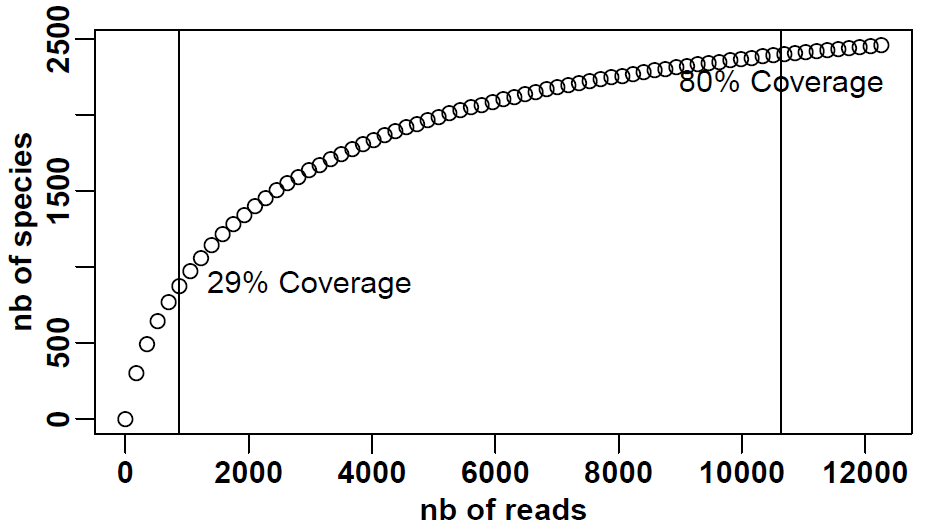
\epsfig{file=../Figures/Rarefaction.ps, clip=, width=.7\textwidth,
      bbllx=43, bblly=39, bburx=570, bbury=340, clip=}
%     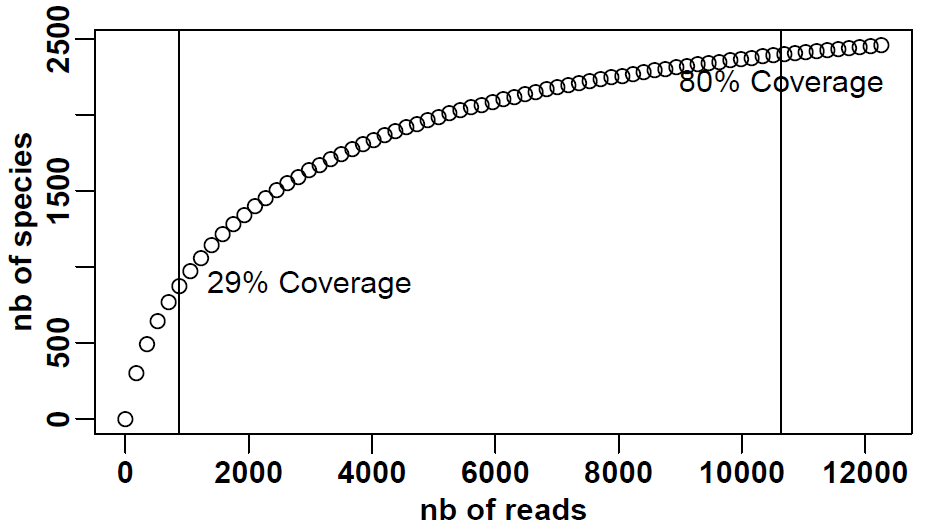
\includegraphics[width=0.7\textwidth, bbllx=43, bblly=39,
%     bburx=570, bbury=340, clip=]{../Figures/Rarefaction.pdf}  
  \end{tabular}
  $$
  }


%====================================================================
\section{Species abundance}
\subsection{An old question}
\frame{ \frametitle{Species abundance}
%==================================================================== 
  \paragraph{An old question:} 
  \begin{itemize} 
  \item Consider a set of individuals sampled in a given area (or
    middle) and classifiy them according to their repsective species;
  \item Denote
    $$
    X_i = \# \text{individuals from species $i$}, \qquad i = 1, .. c
    $$
    where $c$ is the \emphase{number of observed species};
  \item What is the \emphase{total number of species $C$} that are
    present in this area?
  \end{itemize} 

  \bigskip\pause
  \paragraph{Several domains of application:}
  \begin{itemize} 
  \item Ecology: historical problem.
  \item Linguistic: How many words do exist in a given language?
  \item ... \pause
  \item \emphase{Metagenomics}: How many bacterial species (or
    \emphase{genes}) are present in a soil, a human gut or a specific
    marine region?
  \end{itemize} 
}


%====================================================================
\frame{ \frametitle{Exponential family / Conjugate prior}

  \paragraph{Exponential family:}
  $$
  P(\Xbf, \Zbf|\thetabf) \propto \exp[\emphase{\psi(\thetabf)}' \ubf(\Xbf,
  \Zbf)]
  $$
  includes distributions like geometric, Poisson, truncated geometric
  ... but \emphase{not truncated Poisson}. 
  
  (Truncated Poisson can yet be handled using an additional unobserved
  variable.)

  \bigskip\pause
  \paragraph{Conjugate prior.}
  $$
  P(\thetabf) \propto \exp[\emphase{\psi(\thetabf)}' \nubf] 
  $$
  that is 
  \begin{itemize}
  \item Dirichlet for the multinomial distribution ($\Zbf$), 
  \item Gamma for Poisson or Beta for the geometric ($\Xbf|\Zbf$),
  \end{itemize}
  $$
  \Rightarrow \qquad P(\thetabf|\Xbf, \Zbf) \propto
  \exp\{\emphase{\psi(\thetabf)}' [\ubf(\Xbf, \Zbf) + \nubf] \}.
  $$

  }

%====================================================================
\frame{ \frametitle{Variational Bayes E-M}

  \paragraph{Best approximation.} As $P(\thetabf, \Zbf|\Xbf)$ is
  intractable, we look for an approximate distribution $Q(\thetabf,
  \Zbf)$ with a class of 'manageable' ones.

  \bigskip\bigskip\pause
  \paragraph{Factorisable distributions.} When considering the class
  $$
  \Qcal = \{Q(\thetabf, \Zbf) = \emphase{\Qt(\theta)
    \QZ(\Zbf)}\}, 
  $$
  the optimal $Q^* \in \Qcal$ in terms of K�llback-Leibler
  divergence can be recovered via the VB-EM algorithm:
  \begin{eqnarray*}
    \text{'M'-step:} \quad \Qt(\thetabf) 
    & \propto 
    & \exp \left(\phi(\thetabf)'
      \left[ \Esp_{\emphase{\QZ}}u(\Xbf, \Zbf) + \nubf \right]
    \right) \\ 
    \\
    \text{'E'-step:} \quad \QZ(\Zbf)     
    & \propto     
    & \exp ( \Esp_{\emphase{\Qt}}\phi(\thetabf)' u(\Xbf, \Zbf) ]
  \end{eqnarray*}
  \refer{BeG03}

  }

%====================================================================
\subsection{Model averaging}
\frame{ \frametitle{Model averaging}
%==================================================================== 

  \paragraph{Number of components.} 
  \begin{itemize}
  \item The number of components $K$ is unknown and needs to be
    estimated
  \item ... but the existence of a '\emphase{true}' number of
    component is questionable.
  \end{itemize}
  
  \bigskip\pause
  \paragraph{Model averaging.} Instead of choosing the 'best' $K$ we
  rather
  \begin{enumerate}
  \item fit the model for a series of $K = 1 \dots K_\max$:
    $$
    \Qt^*(\thetabf|K)
    $$
  \item and then \emphase{average all models} with weights $w_1, \dots
    w_{K_{\max}}$.
  \end{enumerate}
  
  \bigskip\pause
  Standard Bayesian reasoning indicates that the weights should be
  $$
  \emphase{w_K = P(K|\Xbf)}
  $$
  that can be also approximated using again a variational approach.
  
  }

%====================================================================
%====================================================================
\end{document}
%====================================================================
%====================================================================

  \begin{tabular}{cc}
    \hspace{-.5cm}
    \begin{tabular}{p{.5\textwidth}}
    \end{tabular}
    & 
    \hspace{-.5cm}
    \begin{tabular}{p{.5\textwidth}}
    \end{tabular}
  \end{tabular}

